\subsection{Técnico}
Para acceder, deberá ingresar con un perfil de tipo Técnico, donde luego de iniciar sesión, observará el siguiente menú:

\subsubsection*{Visualiza y gestionar tickets}

\begin{enumerate}
	\item Para acceder, deberá ingresar con un perfil de tipo Técnico, donde luego de iniciar sesión, observará el siguiente menú:
   	\begin{figure}[H]
    \centering
    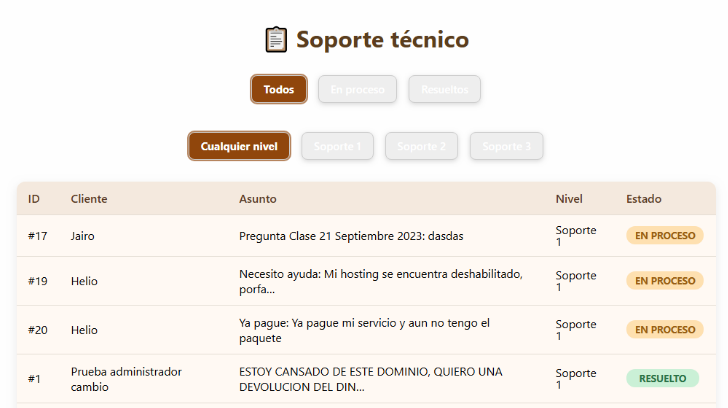
\includegraphics[width=0.75\linewidth]{guiamodulo/tecnico-menu.png}
    \caption{Feed general técnico.}
    \label{fig:tecnico-menu}
    \end{figure}

    \item Donde podrá Visualizar los tickets y editar su estado
    \begin{figure}[H]
    \centering
    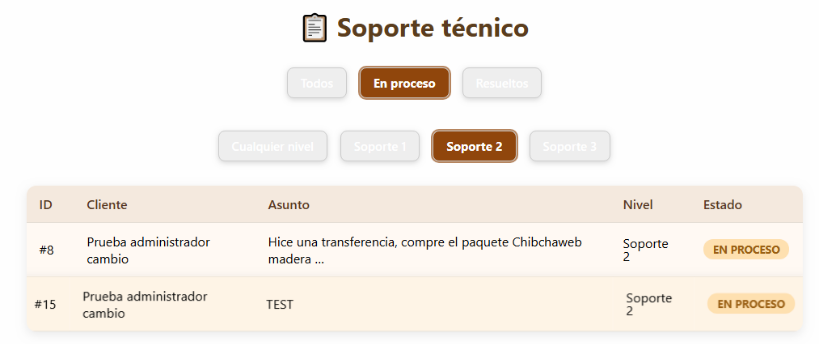
\includegraphics[width=0.75\linewidth]{guiamodulo/tecnico-proceso.png}
    \caption{Feed "En proceso" técnico.}
    \label{fig:tecnico-proceso}
    \end{figure}
\end{enumerate}

\subsection{Coordinador}
Para acceder, deberá ingresar con un perfil de tipo Coordinador sin importar el nivel, donde luego de iniciar sesión, observará el siguiente menú:

\begin{figure}[H]
    \centering
    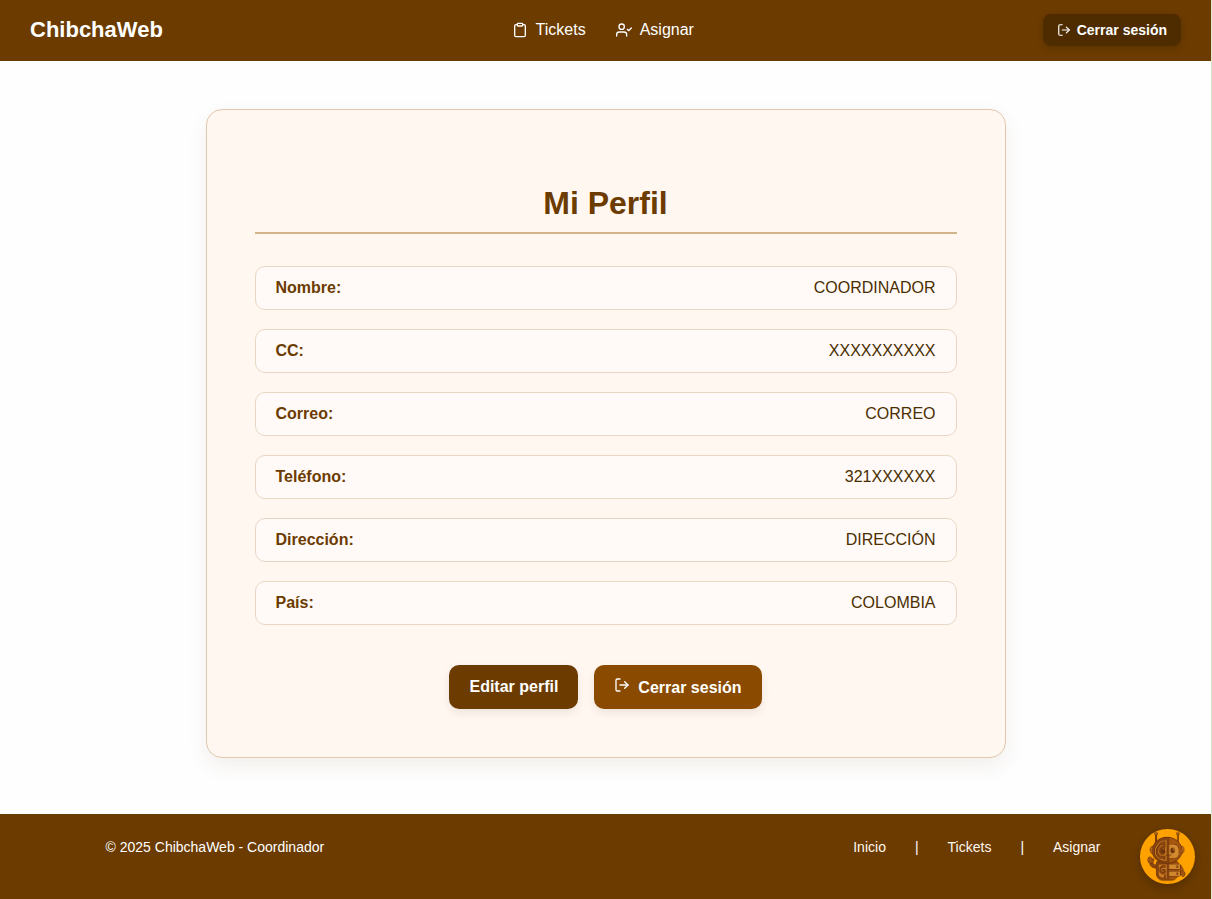
\includegraphics[width=0.75\linewidth]{guiamodulo/perfil-coordinador.png}
    \caption{Perfil Coordinador.}
    \label{fig:perfil-coordinador}
\end{figure}

Con este perfil, podrá realizar las siguientes acciones:

\begin{enumerate}
    \item Gestión de Tickets.
    \item Asignación de tickets.
\end{enumerate}

A continuación se describe como realizar cada una de las acciones:

\subsubsection{Gestión de tickets }
\begin{enumerate}
    \item Dar click en la pestaña "Tickets".
        \begin{figure}[H]
        \centering
        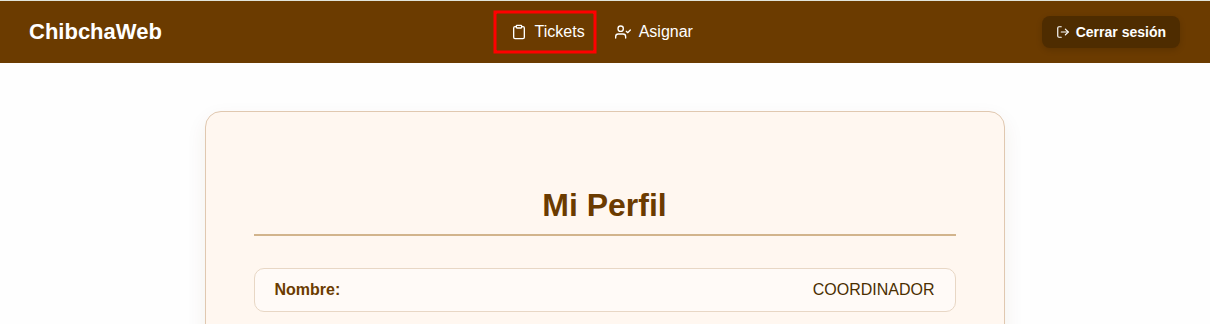
\includegraphics[width=0.8\linewidth]{guiamodulo/navbar-coo-tickect.png}
        \caption{Barra de navegación coordinador, Tickets.}
        \label{fig:navbar-coo-tickect}
        \end{figure}
    \item Allí podrá observar 3 categorias de tickets según el estado en el que se encuentren: Sin asignar, En proceso, Terminado.
        \begin{figure}[H]
            \centering
            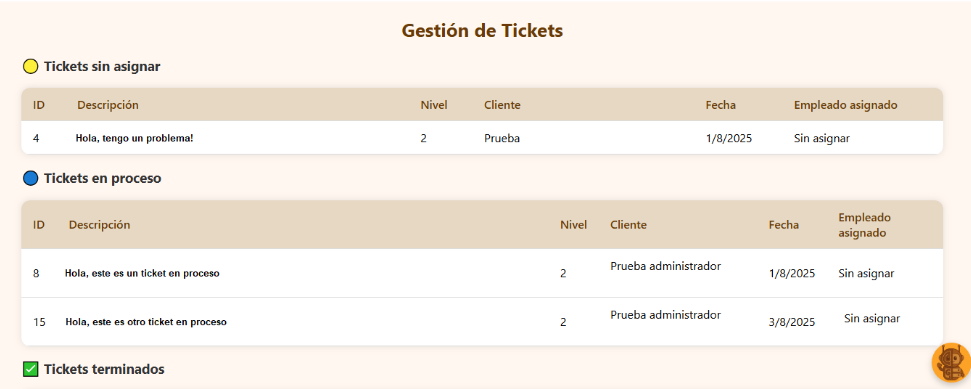
\includegraphics[width=0.8\linewidth]{guiamodulo/coordinador-tickets.png}
            \caption{Feed de tickets del coordinador.}
            \label{fig:coordinador-tickets}
        \end{figure}
\end{enumerate}

\subsubsection{Asignación de tickets }
\begin{enumerate}
    \item Para ello se debe ingresar a “Asignar”, de la siguiente manera:
        \begin{figure}[H]
        \centering
        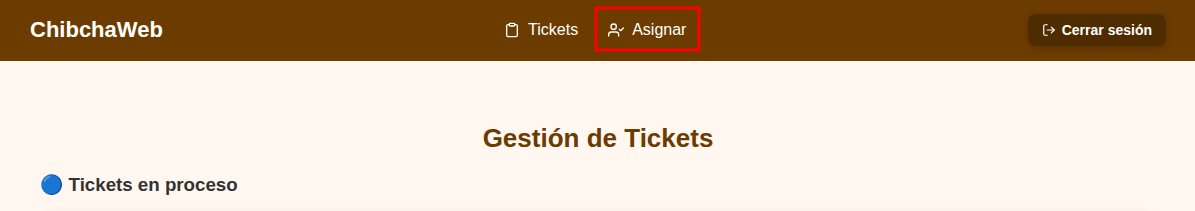
\includegraphics[width=0.8\linewidth]{guiamodulo/navbar-coo-asignar.png}
        \caption{Barra de navegación coordinador, Asignar.}
        \label{fig:navbar-coo-asignar}
        \end{figure}
    \item Donde se encontrarán los tickets disponibles, y podrá asignarlos a un empleado de soporte, o escalarlo.
        \begin{figure}[H]
            \centering
            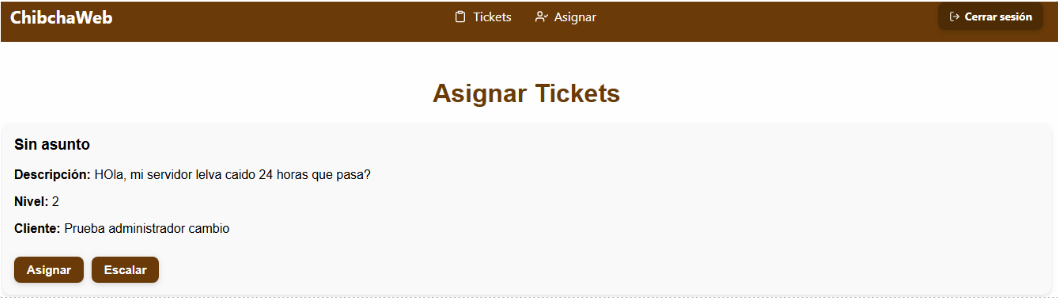
\includegraphics[width=0.8\linewidth]{guiamodulo/coordinador-asignar.png}
            \caption{Enter Caption}
            \label{fig:placeholder}
        \end{figure}
\end{enumerate}


\subsection{Administrador}
Para acceder, deberá ingresar con un perfil de tipo Administrador, donde luego de iniciar sesión, observará el siguiente menú:
\begin{figure}[H]
    \centering
    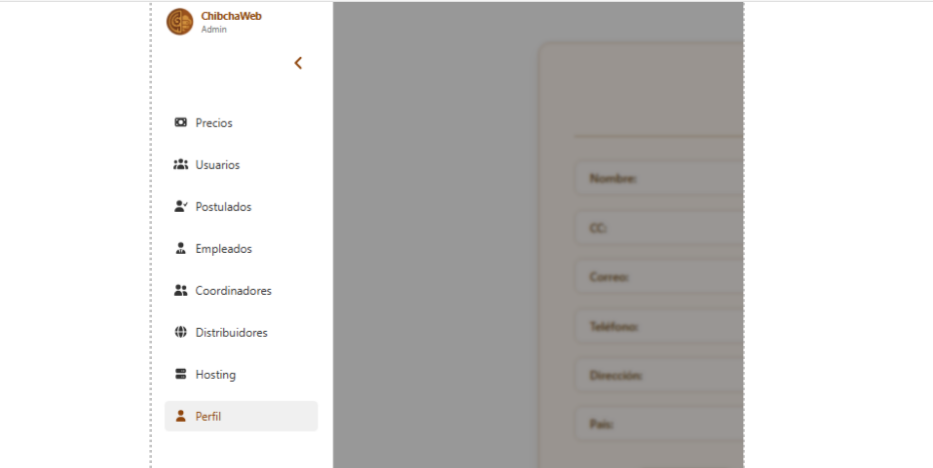
\includegraphics[width=1\linewidth]{guiamodulo/menu-admin.png}
    \caption{Menú Administrador}
    \label{fig:menu-admin}
\end{figure}

Con este perfil, podrá realizar las siguientes acciones:

\begin{itemize}
    \item{Modificar Precios de dominios}
    \item{Gestionar Usuarios}
    \item{Gestionar Empleados}
    \item{Gestionar Distribuidores}
    \item{Gestionar planes de Hosting}
    \item{Gestionar perfil}
\end{itemize}

A continuación, se describen como realizar cada una de ellas

\subsubsection{Modificar Precios de dominios}
\begin{enumerate}
    \item Para realizar esta acción, se debe dar clic en “Precios” del menú del administrador visto en la figura \ref{fig:menu-admin}.
    \begin{figure}[H]
        \centering
        
\includegraphics[width=0.3\linewidth]{guiamodulo/menu-admin-precios.png}
        \caption{Menú Admin, botón Precios}
        \label{fig:menu-admin-precios}
    \end{figure}

    \item Seleccionar la extensión a la que se desea modificar el precio, y editarlo
    \begin{figure}[H]
        \centering
        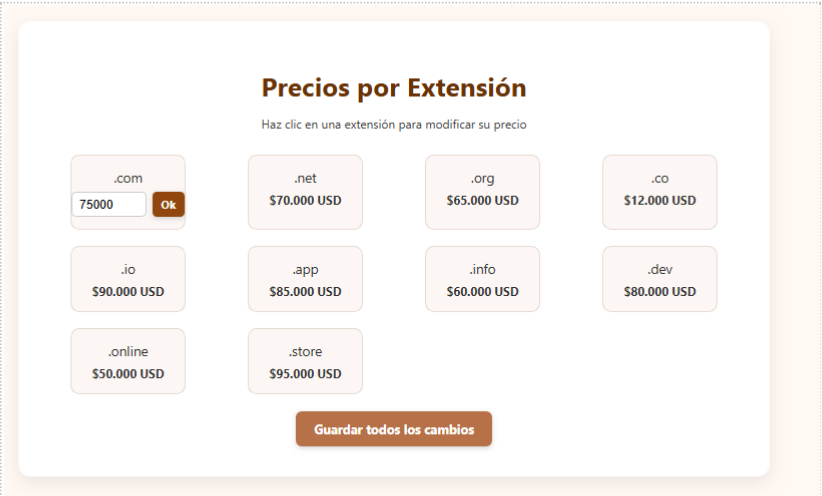
\includegraphics[width=0.7\linewidth]{guiamodulo/mod-precios.png}
        \caption{Modificar precios de por extensión.}
        \label{fig:mod-precios}
    \end{figure}

     \item Seleccionar el botón “Guardar todos los cambios”
    \begin{figure}[H]
        \centering
        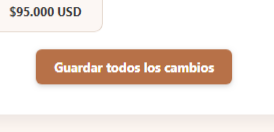
\includegraphics[width=0.4\linewidth]{guiamodulo/mod-precios-guardar.png}
        \caption{Modificar precios de por extensión, guardar.}
        \label{fig:mod-precios-guardar}
    \end{figure}

    \item  Si todo se realizó de la forma correcta, se mostrará el siguiente aviso:
    \begin{figure}[H]
        \centering
        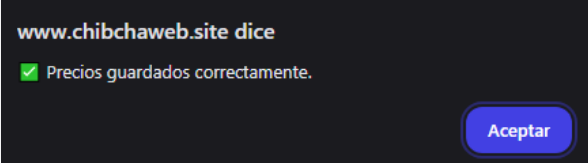
\includegraphics[width=0.75\linewidth]{guiamodulo/mod-precios-aviso.png}
        \caption{Modificar precios de por extensión, notificación.}
        \label{fig:mod-precios-aviso}
    \end{figure}
\end{enumerate}


\subsubsection{Gestionar Usuarios}
\begin{enumerate}
    \item Para realizar esta acción, se debe dar clic en el botón “Usuarios” del menú del administrador visto en la figura \ref{fig:menu-admin}.
visto en la figura
        \begin{figure}[H]
            \centering
            
\includegraphics[width=0.3\linewidth]{guiamodulo/menu-admin-usuarios.png}
            \caption{Mené Admin, botón Usuarios}
            \label{fig:menu-admin-usuarios}
        \end{figure}

    \item Donde podrá buscar y seleccionar los clientes registrados
    \begin{figure}[H]
        \centering
        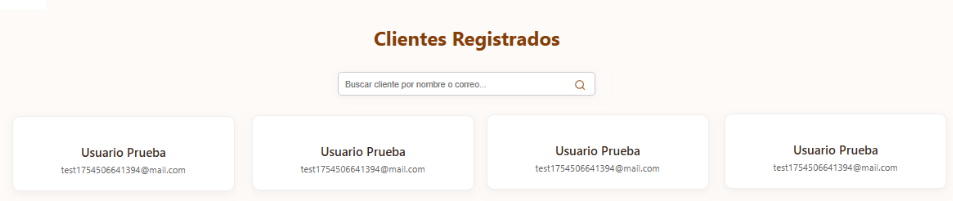
\includegraphics[width=0.8\linewidth]{guiamodulo/admin-usuarios-registrados.png}
        \caption{Admin, usuarios registrados.}
        \label{fig:admin-usuarios-registrados}
    \end{figure}

    \item Accediendo al detalle del cliente, y decidir si editar su información, o eliminar la cuenta
    \begin{figure}[H]
        \centering
        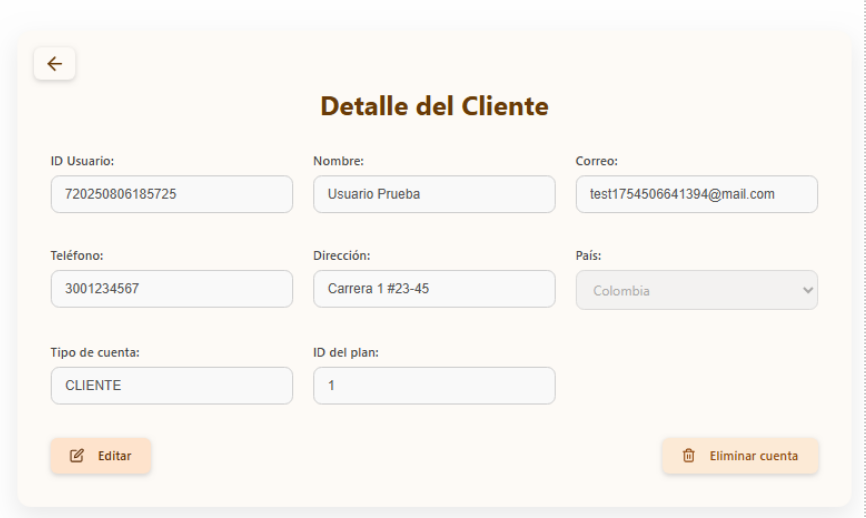
\includegraphics[width=0.75\linewidth]{guiamodulo/admin-usuario-detalle.png}
        \caption{Admin, detalle usuario.}
        \label{fig:admin-usuario-detalle}
    \end{figure}
\end{enumerate}

\subsubsection{Gestionar Postulados}
\begin{enumerate}
    \item Para realizar esta acción, se debe dar clic en “Postulados”
    \begin{figure}[H]
        \centering
        
\includegraphics[width=0.3\linewidth]{guiamodulo/menu-admin-postulados.png}
        \caption{Menú Admin, postulados.}
        \label{fig:menu-admin-postulados}
    \end{figure}

    \item Seleccione el empleado que desea aceptar
    \begin{figure}[H]
        \centering
        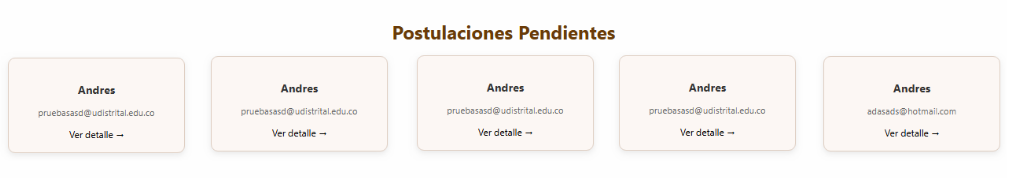
\includegraphics[width=0.8\linewidth]{guiamodulo/admin-postulados.png}
        \caption{Postulados.}
        \label{fig:admin-postulados}
    \end{figure}

    \item Seleccione el nivel de soporte y clic en el boton “Asignar nivel”
    \begin{figure}[H]
        \centering
        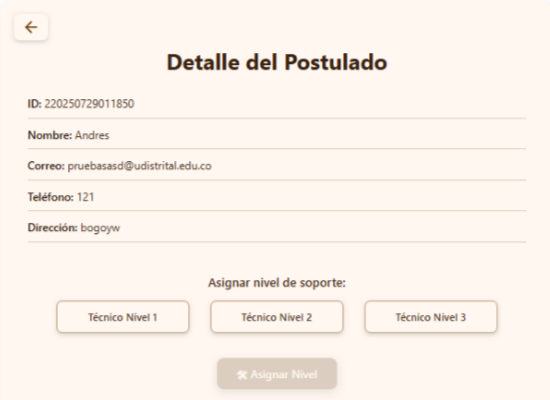
\includegraphics[width=0.6\linewidth]{guiamodulo/admin-postulados-detalle.png}
        \caption{Detalle postulado.}
        \label{fig:admin-postulados-detalle}
    \end{figure}
\end{enumerate}

\subsubsection{Gestionar Empleados}

\begin{enumerate}
\item Para realizar esta acción, se debe dar clic en “Empleados”

\begin{figure}[H]
    \centering
    
\includegraphics[width=0.3\linewidth]{guiamodulo/menu-admin-empleados.png}
    \caption{Menú Admin, empleados.}
    \label{fig:menu-admin-empleados}
\end{figure}

\item  Seleccionar el técnico deseado y dar clic en “Reasignar”

\begin{figure}[H]
    \centering
    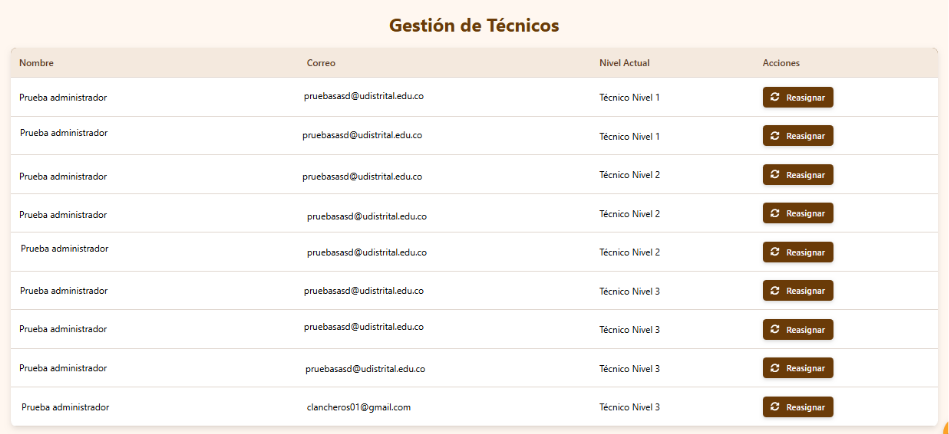
\includegraphics[width=0.7\linewidth]{guiamodulo/gestion-tecnicos.png}
    \caption{Gestión técnicos.}
    \label{fig:gestion-tecnicos.png}
\end{figure}

\item Seleccionar el nuevo nivel de técnico a asignar, y dar clic en “Guardar”

\begin{figure}[H]
    \centering
    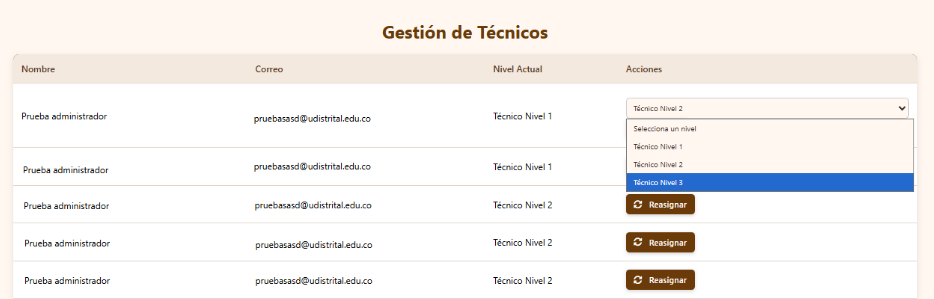
\includegraphics[width=0.7\linewidth]{guiamodulo/gestion-tecnicos-menu.png}
    \caption{Gestión técnicos, selección niveles.}
    \label{fig:gestion-tecnicos-menu.png}
\end{figure}

\item Si todo salió bien, se observará el anuncio de actualización, de la siguiente manera

\begin{figure}[H]
    \centering
    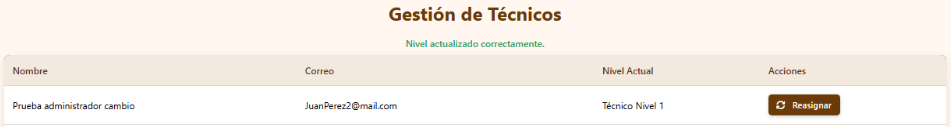
\includegraphics[width=0.7\linewidth]{guiamodulo/gestion-tecnicos-aviso.png}
    \caption{Gestión técnicos, notificación.}
    \label{fig:gestion-tecnicos-aviso.png}
\end{figure}

\end{enumerate}

\subsubsection{Gestionar Coordinadores}

\begin{enumerate}
\item Para realizar esta acción, se debe dar clic en “Coordinadores”

\begin{figure}[H]
    \centering
    
\includegraphics[width=0.3\linewidth]{guiamodulo/menu-admin-coordinadores.png}
    \caption{Menú Admin, coordinadores.}
    \label{fig:menu-admin-coordinadores}
\end{figure}

\item Igual que el punto anterior, se debe seleccionar el nuevo nivel y guardar

\begin{figure}[H]
    \centering
    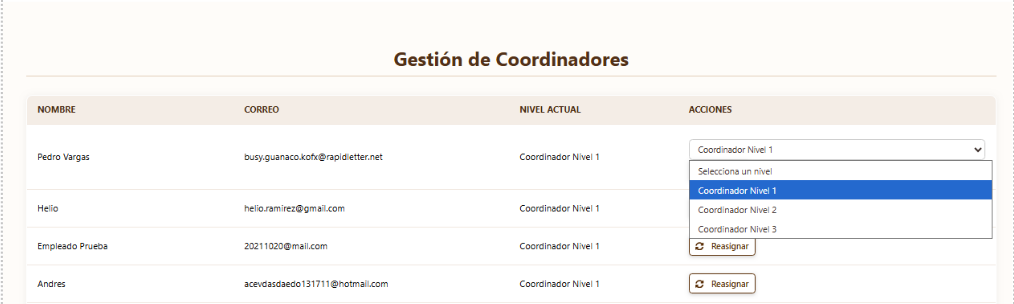
\includegraphics[width=0.7\linewidth]{guiamodulo/gestion-coordinadores.png}
    \caption{Gestión coordinadores.}
    \label{fig:gestion-coordinadores.png}
\end{figure}

\item Si todo salió bien, se observará el anuncio de actualización, de la siguiente manera

\begin{figure}[H]
    \centering
    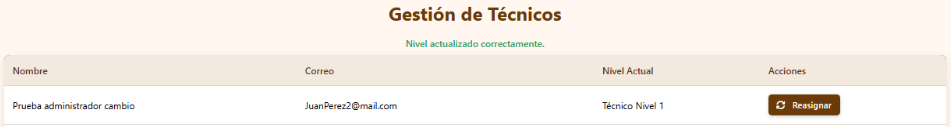
\includegraphics[width=0.7\linewidth]{guiamodulo/gestion-tecnicos-aviso.png}
    \caption{Gestión coordinadores, notificación.}
    \label{fig:gestion-coordinadores-aviso.png}
\end{figure}

\end{enumerate}


\subsubsection{Gestionar Distribuidores}

 \begin{enumerate}
 \item Para realizar esta acción, se debe dar clic en “Distribuidores”
 \begin{figure}[H]
     \centering
     
\includegraphics[width=0.3\linewidth]{guiamodulo/menu-admin-distribuidores.png}
     \caption{Menú Admin, distribuidores.}
     \label{fig:menu-admin-distribuidores}
 \end{figure}

 \item Seleccione el distribuidor a consultar
 \begin{figure}[H]
     \centering
     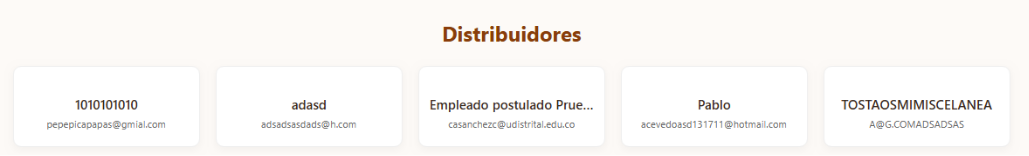
\includegraphics[width=0.7\linewidth]{guiamodulo/gestion-distribuidores.png}
     \caption{Gestión distribuidores.}
     \label{fig:gestion-distribuidores.png}
 \end{figure}

 \item Edite la información del distribuidor
 \begin{figure}[H]
     \centering
     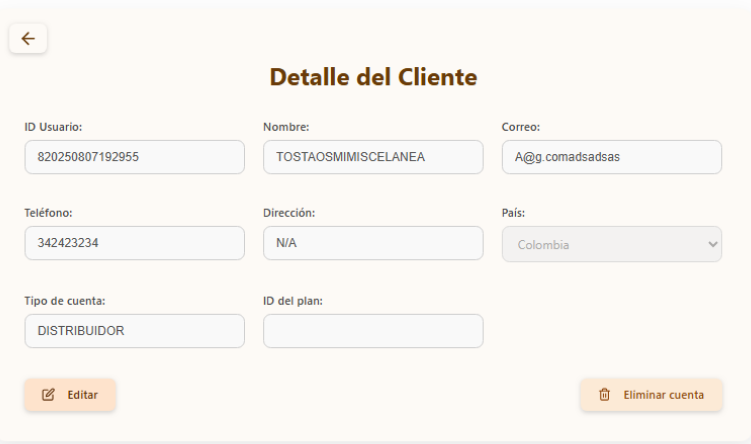
\includegraphics[width=0.7\linewidth]{guiamodulo/gestion-distribuidores-detalle.png}
     \caption{Gestión distribuidores detalle.}
     \label{fig:gestion-distribuidores-detalle.png}
 \end{figure}

 \end{enumerate}


\subsubsection{Gestionar planes de Hosting}

\subsubsection*{Editar paquete de Hosting}

\begin{enumerate}
    \item Para realizar esta acción, se debe dar clic en “Hosting”
    \begin{figure}[H]
        \centering
        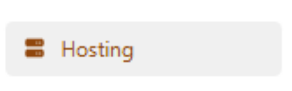
\includegraphics[width=0.3\linewidth]{guiamodulo/menu-admin-hosting.png}
        \caption{Menú Admin, hosting.}
        \label{fig:menu-admin-hosting}
    \end{figure}

    Podrá editar los atributos de los diferentes planes de Hosting, seleccionando la periodicidad y dando clic encima de cada valor

    \begin{figure}[H]
        \centering
        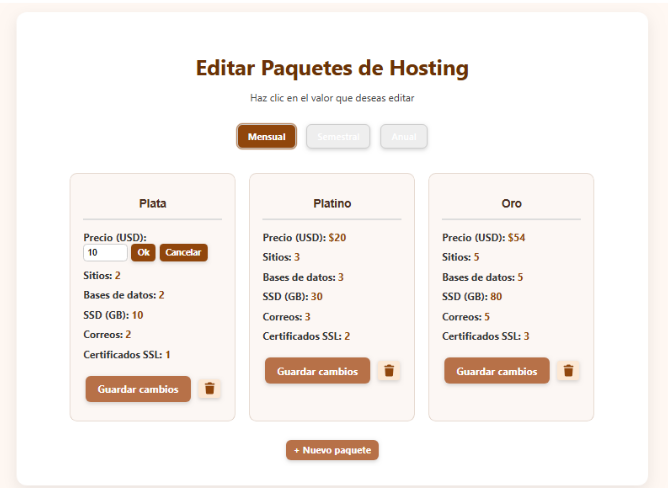
\includegraphics[width=0.7\linewidth]{guiamodulo/gestion-hosting.png}
        \caption{Gestión hosting.}
        \label{fig:gestion-hosting.png}
    \end{figure}

    \item Luego de modificar los valores deseados deber seleccionar “Guardar cambios” en el paquete deseado

    \begin{figure}[H]
        \centering
        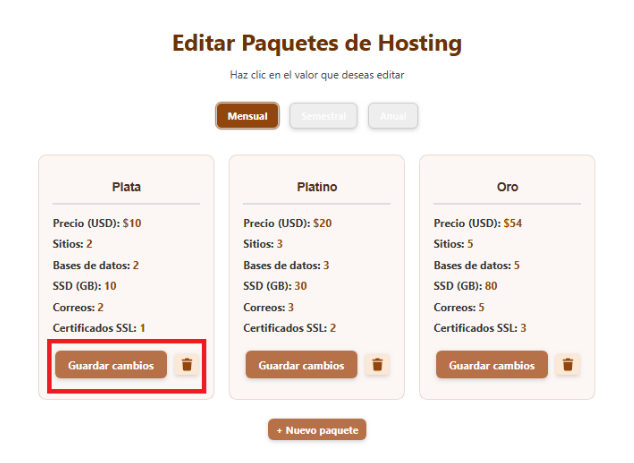
\includegraphics[width=0.7\linewidth]{guiamodulo/gestion-hosting-guardar.png}
        \caption{Gestión hosting, guardar.}
        \label{fig:gestion-hosting-guardar.png}
    \end{figure}

    \item Si todo sale bien, verá el mensaje siguiente

    \begin{figure}[H]
        \centering
        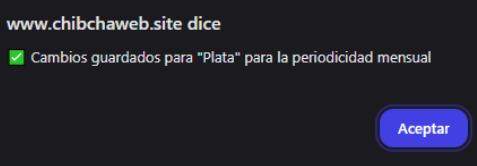
\includegraphics[width=0.4\linewidth]{guiamodulo/gestion-hosting-aviso.png}
        \caption{Gestión hosting, notificación.}
        \label{fig:gestion-hosting-aviso.png}
    \end{figure}

\end{enumerate}

\subsubsection*{Añadir un nuevo paquete de Hosting}
\begin{enumerate}
	\item Desde la vista de Paquete, debe seleccionar la periodicidad e ingresar a “Nuevo Paquete”
	\begin{figure}[H]
        \centering
        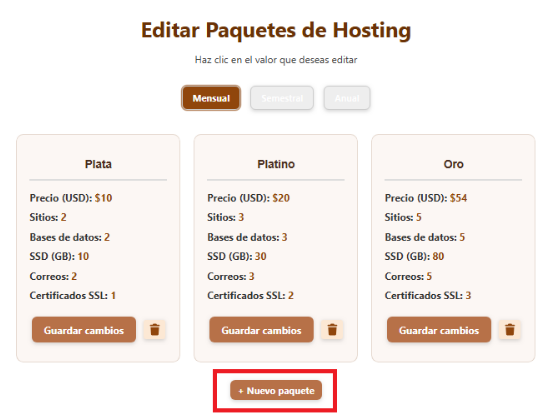
\includegraphics[width=0.7\linewidth]{guiamodulo/gestion-hosting-nuevo.png}
        \caption{Gestión hosting, nuevo paquete.}
        \label{fig:gestion-hosting-nuevo.png}
    \end{figure}

	\item Llene los campos solicitados
	\begin{figure}[H]
        \centering
        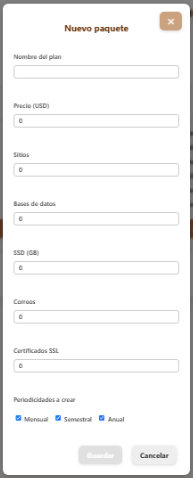
\includegraphics[width=0.2\linewidth]{guiamodulo/gestion-hosting-nuevo-campos.png}
        \caption{Gestión hosting, campos nuevo paquete.}
        \label{fig:gestion-hosting-nuevo-campos.png}
    \end{figure}

    \item De clic en Guardar
\end{enumerate}


\subsubsection {Gestionar perfil }

\begin{enumerate}
\item Para realizar esta acción, se debe dar clic en “Mi perfil”
\begin{figure}[H]
    \centering
    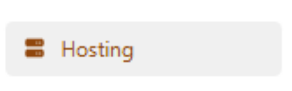
\includegraphics[width=0.3\linewidth]{guiamodulo/menu-admin-hosting.png}
    \caption{Menú Admin, perfil.}
    \label{fig:menu-admin-perfil}
\end{figure}
\end{enumerate}
